\documentclass[runningheads]{llncs}
\usepackage[T1]{fontenc}
\usepackage{amsmath,amssymb,mathtools}
\usepackage{array}
\usepackage{booktabs}
\usepackage{graphicx}
\usepackage{float}
\usepackage{tikz}
\usetikzlibrary{arrows.meta,positioning,decorations.pathreplacing}
\usepackage{hyperref}
\hypersetup{hidelinks}
\usepackage{listings}
\lstset{basicstyle=\ttfamily\footnotesize,columns=fullflexible,keepspaces=true,breaklines=true,xleftmargin=2mm,aboveskip=2pt,belowskip=6pt}
\usepackage{microtype}
\usepackage{needspace}
\usepackage{xcolor}

\newif\ifanonymous
\anonymoustrue

\newcommand{\Rocq}{Rocq}
\newcommand{\coqin}[1]{\texttt{#1}}
\newcommand{\PG}{\mathrm{PGL}(2,7)}
\newcommand{\Unif}{U_G}
\newcommand{\worddist}{\mu^{*L}}
\newcolumntype{L}[1]{>{\raggedright\arraybackslash}p{#1}}
\spnewtheorem*{thmAinf}{Theorem A (informal)}{\bfseries}{\itshape}
\spnewtheorem*{thmBinf}{Theorem B (informal)}{\bfseries}{\itshape}
\spnewtheorem*{thmA}{Theorem A}{\bfseries}{\itshape}
\spnewtheorem*{thmB}{Theorem B}{\bfseries}{\itshape}

\title{Algebraic Specification of Card-Based Cryptographic Protocols in Rocq}
\ifanonymous
  \author{Anonymous}
  \institute{Submission to WADT 2026}
\else
  \author{Cheng-Hui Weng}
  \institute{Nagoya University}
\fi

\begin{document}
\maketitle

\begin{abstract}
Card-based protocols use physical cards to compute with
information-theoretic security. I define a \Rocq{} framework that treats a
finite group, its permutation action, and its shuffle distribution as first-class
parameters. The framework connects group actions to executed traces and
word-shuffle mixing. The main instance uses the action of
$\PG$ on eight projective points.
Under the uniform shuffle distribution, the instance has exact correctness,
the recovery ramp $(t,r,n)=(3,7,8)$, and perfect view privacy for
coalitions of at most three players, which interpreter soundness transports
to the executed traces. These privacy results hold for a uniform Boolean
secret, a fixed encoded representative, and passive adversaries, with the
verifier learning the secret and with active security, security after the
reveal, and composition outside the model. Because no single physical move samples a uniform group element, I
analyze a finite implementation that draws a uniform word of length 200
over five generator letters. A checked fiber-counting certificate proves that
the resulting shuffle distribution is within $L_1$ distance $2^{-40}$ of the
uniform group distribution. This word-shuffle theorem transfers to single-card
marginals and to a product with any secret prior. Transport theorems therefore bound approximate coalition-view and
executed-trace privacy by $2^{-39}$ under the word distribution.
A five-card family and two spectral siblings show which algebraic,
operational, privacy, and mixing arguments the framework reuses, the
spectral siblings importing one analytic gap premise as their only
assumption beyond the classical principles used throughout.
\end{abstract}

\section{Introduction}\label{sec:introduction}

Card-based cryptography uses face-down physical cards to compute functions
without computational assumptions. A shuffle hides a permutation, while a
reveal exposes selected card faces. Information-theoretic security requires
the resulting observation distribution to hide the protected secret. Den Boer's
five-card protocol began this line of work~\cite{denBoer1989}. Later protocols
reduced card counts and broadened the class of supported
computations~\cite{MizukiSone2009,MizukiSone2012,KochWalzerHartel2015}.

Mechanized analysis must connect the physical operations to their probability
distributions. Koch, Schrempp, and Kirsten use software bounded model checking to
search finite protocol spaces and check lower bounds~\cite{Koch2019}.
Their method automates checks over a bounded state space, and a bound
checked for one finite protocol space says nothing about every
$t$-transitive group action. The development\footnote{The companion
artifact contains the source, theorem index, assumption report, and build
instructions.} in this article instead uses a proof assistant whose generic
theorems quantify over the group, the action, and the shuffle distribution,
and it states reusable dealer distributions, participant views, and
executed traces. It combines a group-parametric model with perfect trace
privacy and a checked word-shuffle mixing bound.

Two shuffle distributions organize the analysis. The uniform distribution
on the shuffle group is the ideal object of the security proofs. No dealer
samples a uniform group element in one physical move. A dealer instead
repeats elementary moves drawn from a small generator alphabet, and the
repeated moves follow what I call a word distribution over the generators
of the group. In the five-card family the moves are genuine cuts, while
the $\PG$ letters are group generators whose physical realization I do not
claim. The group parameters pay for this connection. Transitivity of the
action yields coalition privacy, and generation by a small alphabet yields
a finite executable shuffle. In this paper I prove the security results in the uniform-shuffle model of Section~\ref{sec:model} and then
prove that the word distribution approximates it.

Overall, this work contributes a group-parametric framework whose main
instance carries two machine-checked security results.

\begin{thmAinf}
The $\PG$ instance recovers the secret from all eight endpoints for every
group element. Under the uniform shuffle distribution, with a uniform
Boolean secret and the fixed representative dealer, it has recovery
parameters $(t,r,n)=(3,7,8)$ and perfect view and executed-trace privacy
against every passive coalition of at most three
players.\footnotemark
\end{thmAinf}
\footnotetext{Formal statement at the end of
Section~\ref{sec:exact}. The constituent formalized results are
\coqin{pgl27\_run\_recovers}, \coqin{pgl27\_reveal\_ambiguous},
\coqin{pgl27\_seven\_reveal\_class}, \coqin{pgl27\_view\_leak\_k4},
\coqin{pgl27\_view\_indep}, and \coqin{pgl27\_coalition\_trace\_secrecy} in
\path{pgg-smc/instances/pgl27}.}

\begin{thmBinf}
The 200-letter word shuffle over the five generator letters is within
$L_1$ distance $2^{-40}$ of the uniform shuffle distribution. For
the fixed representative dealer, the coalition view distributions at the two
secrets are within $L_1$ distance $2^{-39}$ for every passive
coalition of at most three players, and the executed coalition traces
satisfy the same bound. Executed correctness holds for every
word.\footnotemark
\end{thmBinf}
\footnotetext{Formal statement at the end of
Section~\ref{sec:mixing}. The constituent formalized results are
\coqin{pgl27\_word\_mixing}, \coqin{pgl27\_word\_view\_indist},
\coqin{pgl27\_word\_trace\_indist}, and \coqin{pgl27\_word\_run\_recovers} in
\path{pgg-smc/instances/pgl27}.}

There are five contributions in this work.
\begin{itemize}
\item I give a common \Rocq{} interface for a finite group, its permutation
  action, the shuffle distribution, reconstruction, participant views, and executed
  traces.
\item I verify the den Boer~\cite{denBoer1989} and the Kim and
  \c{C}etinkaya~\cite{KimCetinkaya2025} five-card protocols in \Rocq{} as
  one profile at bias $\varepsilon$, in the sense of
  Section~\ref{sec:framework}: executed-run correctness of the conjunction
  output, executed-trace secrecy for a single corrupted player, and
  input-hiding given the announced output.
\item I prove exact mutual-information leakage values for every reveal
  pattern of the five-card family, recover den Boer's perfect dealing
  bound at bias zero, and check in the kernel a seven-cut single-card
  bound of $2^{-40}$ at bias $1/100$.
\item I prove correctness, the recovery ramp, coalition-view privacy, and
  executed-trace secrecy for the $\PG$ instance under the uniform shuffle
  distribution.
\item I prove an $L_1$ bound between a 200-letter generator-word distribution
  and the uniform group distribution.\footnote{The $L_1$ distance is
  $\lVert P-Q\rVert_1=\sum_x\lvert P(x)-Q(x)\rvert$, which is called
  variation distance in the formal development, with maximum value 2. The common total
  variation distance is half of it. An $L_1$ bound of $2^{-40}$ therefore
  bounds every observer's distinguishing advantage by $2^{-41}$. The
  paper's security number is the one derived from the coalition-view
  bound: the $2^{-39}$ view distance of Theorem B bounds every observer's
  distinguishing advantage by $2^{-40}$. The $2^{-41}$ figure concerns
  only the group-element mixing distance.} The proof
  also transfers the bound to card
  endpoints and secret-prior product distributions.
\end{itemize}

Section~\ref{sec:model} fixes the protocol flow, the two distributions, and
the security scope. Section~\ref{sec:framework} presents the framework components used by
the proofs. Section~\ref{sec:fivecard} instantiates them on the five-card
family, where the deck is small enough for direct case analysis.
Sections~\ref{sec:pgl} and~\ref{sec:exact} construct the $\PG$ instance,
where deck enumeration no longer suffices and three-transitivity carries
the privacy proofs, ending in Theorem A. Section~\ref{sec:mixing} proves
the word-shuffle results, ending in Theorem B, because a physical dealer
repeats elementary moves rather than sampling one uniform group element. Section~\ref{sec:instances} compares the sibling instances and
states the trust base. Section~\ref{sec:related} places the results among
related work. Section~\ref{sec:conclusion} states the remaining extensions
and other future directions.

\section{Protocol and Security Model}\label{sec:model}

A run of the protocol handles one secret and a deck of face-down cards. A
dealer encodes the secret as a valid arrangement of the deck. The dealer
then samples a shuffle from a finite group and rearranges the deck by its
permutation action. Each player receives the card at one position. The
players reveal their cards to a verifier, and the verifier decodes the
secret from the revealed arrangement. Each instance section shows its own
run as a flow diagram.

Security rests on the shuffle alone, because the dealer's encoding of
the secret is fixed and the shuffle carries all the randomness. A player
sees one card, and a coalition sees the cards at its positions. The shuffle spreads every small
coalition view over many arrangements, and the privacy theorems make this
spreading exact. The rest of this section states the same flow as
probability distributions.

The framework describes a protocol by the data
\begin{equation}
  (G,\rho,\mu;R), \qquad U_G, \qquad \mu^{*L}.
  \label{eq:model-data}
\end{equation}
Here $G$ is a finite shuffle group. The representation
$\rho:G\to S_n$ acts on $n$ card positions. The distribution $\mu$ selects one
generator letter, and $R$ is the real closed field used for probabilities.
The distribution $U_G$ is uniform on $G$. I write $\mu^{*L}$ for the word distribution at length $L$: the
distribution of the group element obtained by evaluating $L$ independent
letters.

A dealer samples a secret $S$ and a valid dealt arrangement $D$. The action
of a sampled shuffle $g$ produces the arrangement $\rho(g)D$. Position $i$
of the shuffled arrangement holds the card that $D$ places at position
$\rho(g)(i)$. Player $i$
observes a view $V_i$ derived from the card at position $i$. A coalition
$C\subseteq\{0,\ldots,n-1\}$ observes the joint view
\begin{equation}
  V_C=(V_i)_{i\in C}.
  \label{eq:coalition-view}
\end{equation}
The interpreter executes the dealer, player, and verifier processes. It
records each value received by a process. The resulting record is called the
executed trace $T_i$, and $T_C=(T_i)_{i\in C}$ is called the coalition
trace. The
verifier receives all endpoints and applies the decoder. It therefore learns
$S$ by design.

The following player process makes this execution model
concrete.\footnote{Formalized in
\path{pgg-smc/protocol/card_exchange_pismc.v} as
\coqin{exchange\_dealer}, \coqin{exchange\_player}, and
\coqin{exchange\_verifier}.}

\begin{lstlisting}
Definition exchange_player (i : 'I_T)
    : sproc pgg_dtype data (player_idx i) :=
  \pi{ Receive<dealer_idx> #my_hand =>
     Receive<dealer_idx> $shuffle_idx =>
     Reveal<verifier_idx> &(nth ord0 my_hand shuffle_idx) ;
     Finish }.
\end{lstlisting}

In the listing, \coqin{\#} marks a dealt hand, \coqin{\$} marks the
public shuffle index, and \coqin{\&} marks a card position. The player
receives the hand and the index, selects one entry, and reveals it to the
verifier. The verifier receives this entry as its observation. The interpreter
records both received values in the player's trace.
The trace theorem therefore concerns the execution of this process. Its
content is interpreter soundness: under the trace-lifting hypothesis the
recorded trace and the static view determine each other, so the operational
execution reveals nothing beyond the static view, and view privacy
transports to the trace rather than being proved a second time.

The primary execution distribution samples a uniform Boolean secret and
deals one fixed representative arrangement $D_s$ for each secret $s$. It
then applies an independent uniform shuffle. I call this the fixed
representative dealer, and it is the dealer of the headline theorems. An
all-decks dealer instead
samples a uniform valid arrangement in the selected secret class before the
shuffle. Both execution distributions use a uniform Boolean prior.

The security theorems concern passive, honest-but-curious adversaries. A
corrupted player follows the protocol and retains its view and executed
trace. Perfect coalition privacy states that $S$ and $V_C$ are independent.
Perfect trace privacy states
\begin{equation}
  H(S\mid T_C)=H(S).
  \label{eq:trace-privacy}
\end{equation}

The protected object is a dealt secret, as in a secret-sharing
scheme~\cite{Shamir1979}. The dealer holds the secret, the players hold
card observations in place of shares, and privacy bounds what coalitions of
curious players learn. The protocol has no private player inputs. Active
deviation, security after the verifier's reveal, and composition across
executions are outside the model.

The model described so far applies one uniform group element, and I call
it the uniform-shuffle model. A second model describes the dealer
performing the shuffle as a sequence of elementary moves drawn from the
generator alphabet. I call this the
word-shuffle model. It
replaces $U_G$ by $\mu^{*L}$. I measure two distributions $P$
and $Q$ by the $L_1$ distance
\begin{equation}
  \lVert P-Q\rVert_1=\sum_x\lvert P(x)-Q(x)\rvert.
  \label{eq:l1-definition}
\end{equation}

The model observes the word shuffle only through its product. The dealer
performs the 200 physical moves and no party records an intermediate
arrangement. This assumption is structural in the formalization. The dealer process takes a list of alternative cuts and deals one hand
per cut. A word hence enters the execution only through its evaluated
group element. The uniform-shuffle model makes the same assumption, since its single
uniform shuffle is likewise unobserved.

Figure~\ref{fig:models} separates the proved paths for the two distributions. The
lower path reaches approximate coalition-view and executed-trace privacy at
$2^{-39}$.
\begin{figure}[t]
  \centering
  % Drawn at true document font sizes; the picture is never scaled.
  % It is a little wider than the text block, so it is centred by hand.
  \makebox[\linewidth][c]{%
  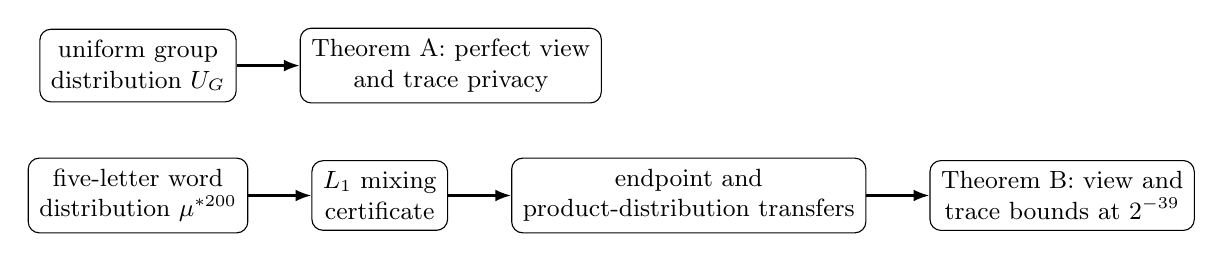
\begin{tikzpicture}[
      node distance=7mm and 8mm,
      box/.style={draw,rounded corners,align=center,inner sep=4pt,
                  font=\small},
      arr/.style={-{Latex[length=2mm]},thick}]
    \node[box] (uniform) {uniform group\\distribution $U_G$};
    \node[box,right=of uniform] (exact) {Theorem A: perfect view\\and trace privacy};
    \draw[arr] (uniform) -- (exact);

    \node[box,below=of uniform] (word) {five-letter word\\distribution $\mu^{*200}$};
    \node[box,right=of word] (lone) {$L_1$ mixing\\certificate};
    \node[box,right=of lone] (transfer) {endpoint and\\product-distribution transfers};
    \node[box,right=of transfer] (privacy)
      {Theorem B: view and\\trace bounds at $2^{-39}$};
    \draw[arr] (word) -- (lone);
    \draw[arr] (lone) -- (transfer);
    \draw[arr] (transfer) -- (privacy);
  \end{tikzpicture}}
  \caption{The two proof paths and the two headline theorems. The upper
  path ends in Theorem A. The lower path transports the mixing certificate
  to Theorem B.}
  \label{fig:models}
\end{figure}

\section{Framework and Generic Theorems}\label{sec:framework}

\subsection{Framework Architecture}

Every instance in this paper supplies the same kinds of data: a group
with its action and generators, a secret type, the layout of a run, a
shuffle-security bound, and a decoder. The framework therefore gathers
these five choices into one record, the record type
\coqin{MonodromyProfile}, in order to reuse one executable protocol
across instances.
The generic theorems of this section take their hypotheses directly, and
the privacy theorem is additionally packaged once at the record level, so a
profile that satisfies the transitivity and distinct-deck obligations
inherits coalition privacy as one instantiation. The
record carries the data of Equation~\ref{eq:model-data} into the
executable protocol. Here $R$ is the real closed field of
Equation~\ref{eq:model-data}, not a protocol datum. The finite algebraic
structures use Mathematical Components~\cite{MathComp}, and
Table~\ref{tab:bridge} maps each model datum to its record role and to the
values the $\PG$ instance supplies.

In the vocabulary of algebraic specification, the record type is a
parameterized loose specification: its fields are the signature, its stated
obligations are the axioms, and an instance that supplies the fields and
discharges the obligations is a model of the
specification~\cite{GoguenBurstall1992,SannellaTarlecki2012}. The five
instances of this paper are five such models, and the relation between the
uniform-shuffle model and its word-shuffle implementation is an approximate
refinement whose distance the $L_1$ bounds of Section~\ref{sec:mixing}
quantify. The record's name borrows monodromy for the way one run
transports the deal along a group element, and prose outside code contexts
says profile record. The specification admits further models beyond the
five of this paper: the affine group $\mathrm{AGL}(1,7)$, which carries
any ordered pair of distinct positions to any other by exactly one
element, and $\mathrm{PGL}(2,11)$ at the present three-transitive
parameters are the natural next instances.

\begin{table}[H]
  \centering
  \small
  \begin{tabular}{@{}L{.26\linewidth}L{.36\linewidth}L{.30\linewidth}@{}}
    \toprule
    Model datum & Record role & $\PG$ instance supplies \\
    \midrule
    layout of a run & dealer, player, and verifier processes & eight
      players, one card each \\
    $(G,\rho)$ with $\mu$ or $U_G$ & endpoint bound for the shuffle
      distribution & three-transitive action, word bound \\
    decoder & reconstruction against the action & orbit-class decoder \\
    all of the above & one packaged protocol instance & the $\PG$ profile \\
    \bottomrule
  \end{tabular}
  \caption{From model data to framework records. In the sources the four
  roles are \coqin{PGGInterface}, \coqin{SecurityWitness},
  \coqin{ReconPlug}, and \coqin{MonodromyProfile}.}
  \label{tab:bridge}
\end{table}

The table identifies the role of each component.
Figure~\ref{fig:framework-architecture} shows how the components and
supporting records depend on one another, and how the profile determines
the executable protocol.

\begin{figure}[H]
  \centering
  % Drawn at true document font sizes; the picture is never scaled.
  % It is a little wider than the text block, so it is centred by hand.
  \makebox[\linewidth][c]{%
  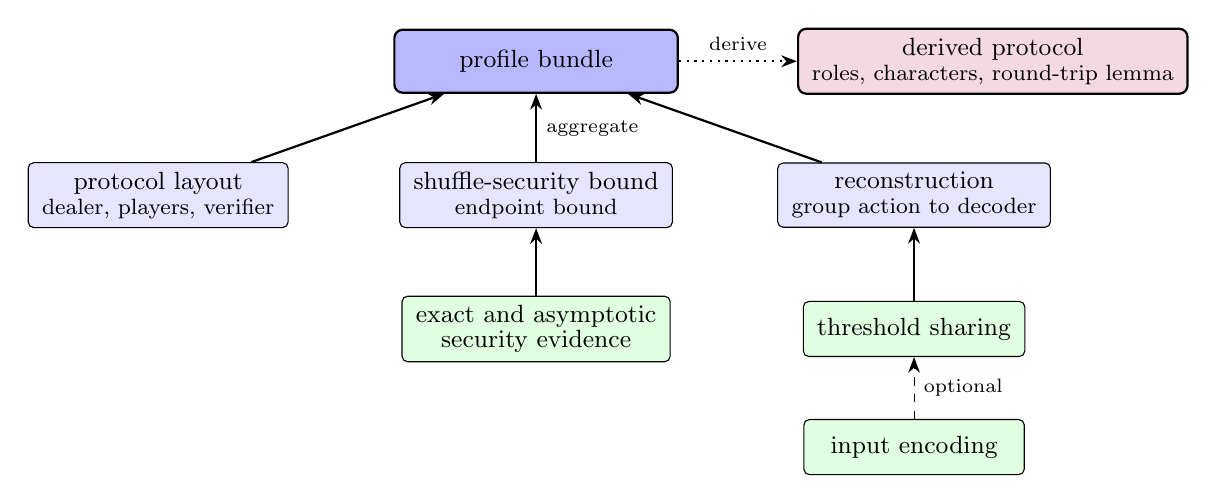
\begin{tikzpicture}[
      every node/.style={font=\small},
      supportbox/.style={
        rectangle, draw, rounded corners=2pt, inner xsep=5pt,
        minimum width=2.8cm, minimum height=0.7cm,
        align=center, fill=green!12
      },
      compbox/.style={
        rectangle, draw, rounded corners=2pt, inner xsep=5pt,
        minimum width=3.2cm, minimum height=0.8cm,
        align=center, fill=blue!10
      },
      bundlebox/.style={
        rectangle, draw, thick, rounded corners=3pt, inner xsep=5pt,
        minimum width=3.6cm, minimum height=0.8cm,
        align=center, fill=blue!28
      },
      derivedbox/.style={
        rectangle, draw, thick, rounded corners=3pt, inner xsep=5pt,
        minimum width=3.6cm, minimum height=0.8cm,
        align=center, fill=purple!15
      },
      arr/.style={-{Stealth[length=2mm]}, thick},
      darr/.style={-{Stealth[length=2mm]}, dashed},
      deparr/.style={-{Stealth[length=2mm]}, dotted, thick}
    ]

    % ===== Bottom: supporting records =====
    \node[supportbox] (ie) at (9.6, 0) {input encoding};
    \node[supportbox] (se) at (4.8, 1.5) {exact and asymptotic\\[-2pt]
      security evidence};
    \node[supportbox] (ts) at (9.6, 1.5) {threshold sharing};

    % ===== Middle: the three component records =====
    \node[compbox] (pi) at (0, 3.2) {protocol layout\\[-2pt]
      \footnotesize dealer, players, verifier};
    \node[compbox] (sw) at (4.8, 3.2) {shuffle-security bound\\[-2pt]
      \footnotesize endpoint bound};
    \node[compbox] (rp) at (9.6, 3.2) {reconstruction\\[-2pt]
      \footnotesize group action to decoder};

    % ===== The aggregate and what it derives =====
    \node[bundlebox] (mp) at (4.8, 4.9) {profile bundle};
    \node[derivedbox] (pr) at (10.6, 4.9) {derived protocol\\[-2pt]
      \footnotesize roles, characters, round-trip lemma};

    % ===== Arrows: supporting records into components =====
    \draw[darr] (ie) -- (ts) node[midway, right, font=\scriptsize] {optional};
    \draw[arr] (se) -- (sw);
    \draw[arr] (ts) -- (rp);

    % ===== Arrows: components into the bundle, bundle into the protocol =====
    \draw[arr] (pi) -- (mp);
    \draw[arr] (sw) -- (mp)
      node[midway, right, font=\scriptsize] {aggregate};
    \draw[arr] (rp) -- (mp);
    \draw[deparr] (mp) -- (pr)
      node[midway, above, font=\scriptsize] {derive};
  \end{tikzpicture}}
  \caption{Architecture of the group-parametric card-protocol framework.
  Blue boxes are profile records, green boxes are supporting records, and
  the purple box is the derived protocol. Solid arrows are required
  dependencies, the dashed arrow is optional, and the dotted arrow is
  derivation.}
  \label{fig:framework-architecture}
\end{figure}

I call a filled \coqin{MonodromyProfile} a profile. Packing these
components in one profile keeps the participants, verifier,
recovery map, privacy threshold, and shuffle bound tied to the same
instance. Each profile supplies proofs of the following three obligations.
\begin{itemize}
\item Every single card position lands close to uniform: \coqin{sw\_bound}
  bounds the distance of each position's endpoint distribution from the
  uniform distribution by \coqin{sw\_bound\_eps}.
\item The threshold scheme recovers and hides: \coqin{ts\_correct} decodes
  every valid share tuple to its secret, and \coqin{ts\_private} gives
  every coalition below the threshold a share pattern that is equally
  consistent with either secret.
\item Reconstruction is shuffle-invariant: for any allowed shuffle and any
  valid share tuple, \coqin{rp\_recon\_invariant} states that permuting the
  shares by the shuffle leaves the recovered secret unchanged.
\end{itemize}

The layout supplies the executable processes described in
Section~\ref{sec:model}. The group action and shuffle distribution fix the
dealing rule and endpoint bound. The reconstruction component chooses the
decoder, so profiles over the same group can use different reconstruction
schemes.

The record that carries the shuffle distribution and its endpoint bound
is called the security witness. It can carry exact evidence, asymptotic
evidence, or both. Table~\ref{tab:witness-mechanism} shows the combinations used by the
five instances in this paper. For example, the den Boer row fills only
the exact slot, since one uniform cut already gives the exact endpoint
distribution. The $\PG$ row also fills only the exact slot. The
word-shuffle bound of Theorem~B is proven in Section~\ref{sec:mixing} but
is not registered in the record's asymptotic slot, so the table reflects
the record contents and Theorem~B's evidence lives outside the witness
record.

\begin{table}[t]
  \setlength{\tabcolsep}{6pt}
  \centering
  \small
  \begin{tabular}{@{}llL{.32\linewidth}L{.20\linewidth}@{}}
    \toprule
    Exact slot & Asymptotic slot & Mechanism & Realized by \\
    \midrule
    present & absent & exact equality at $\varepsilon=0$ under the uniform
      group distribution & den Boer, $\PG$ \\
    present & present & exact count with geometric decay in the word
      length & Kim \\
    absent & present & spectral certificate with an imported gap premise
      & $S_5$, $S_5\times S_5$ \\
    \bottomrule
  \end{tabular}
  \caption{Realized combinations of the security witness's two optional
  slots. Section~\ref{sec:mixing} treats the word-shuffle counterpart of
  the $\PG$ row, Section~\ref{sec:fivecard} proves the den Boer and Kim
  rows, and Table~\ref{tab:instances} records the per-instance evidence.}
  \label{tab:witness-mechanism}
\end{table}

With an \coqin{InputEncoding}, the flow gains a phase that I call the
commit prologue. It collects the players' inputs and assembles the dealt
deck from them, so the same flow evaluates a function of committed
inputs. The realized encoding is den Boer's. Its
orbit obligation places the assembled layouts of equal-output inputs in one
shuffle orbit. This property relates different inputs that produce the same
result. Correctness uses two other facts: the assembled layout is valid, and
reconstruction is invariant under every allowed shuffle. It follows that the
shuffled layout reconstructs the intended output. The Kim variant reuses the
den Boer program unchanged. With an empty input list
the prologue reduces by computation to the plain dealer, which is the
secret-sharing case, and the $\PG$ instance passes exactly this empty
list. Section~\ref{sec:fivecard} realizes the committed-input flow, and
the instance table of Section~\ref{sec:instances} records the full
comparison.

Section~\ref{sec:fivecard} shows how one instance fills these components.
Once the data are packaged, the reusable security arguments depend on
mathematical hypotheses rather than the record representation. The next
subsection states these arguments directly.

\subsection{Generic Theorems}

The first generic theorem yields coalition privacy from transitivity. An
instance discharges its hypothesis by exhibiting a $t$-transitive action on
decks of distinct cards, as Section~\ref{sec:pgl} does for $t=3$.

\begin{theorem}[Generic coalition privacy\footnotemark]\label{thm:generic-privacy}
\footnotetext{Formalized in \path{pgg-smc/reconstruct/transitivity_privacy.v} as
\coqin{ttrans\_view\_indep\_gen}.}
Let $G$ act $t$-transitively on the card positions. Let $S$ be a Boolean
secret with any prior, and suppose that every encoded deck has distinct
cards. If $g$ is uniform on $G$, then
\[
  S \mathrel{\perp\!\!\!\perp} V_C
\]
for every coalition $C$ with $|C|\leq t$.
\end{theorem}

Theorem~\ref{thm:generic-privacy} is also stated once at the record level.
One statement quantifies over any profile: if the group of position
permutations realized by the profile's action is $t$-transitive and every
encoded deck has distinct cards, then the view of every coalition of at
most $t$ positions is independent of the secret, under the record's
share-count and deck-length compatibility premise.\footnote{\coqin{profile\_view\_indep} in
\path{pgg-smc/reconstruct/transitivity_privacy.v}, discharged by the $\PG$
instance as \coqin{pgl27\_view\_indep\_via\_profile} in
\path{pgg-smc/instances/pgl27/pgl27_profile_privacy.v}. The derived
corollary restates the instance's view independence verbatim.} The $\PG$
instance discharges the two obligations with its three-transitivity lemma
and its distinct-deck lemma. Both obligations are necessary rather than
decorative. Weakening the coalition bound to $t+1$ is refuted at the $\PG$
instance by the explicit four-position coalition of
Section~\ref{sec:pgl}, and dropping the distinct-deck
obligation is refuted by a profile over the same group whose encoder deals
one constant card to every position and leaks the secret to a single
position.\footnote{\coqin{profile\_view\_indep\_sharp} and
\coqin{profile\_distinct\_deck\_necessary} in
\path{pgg-smc/instances/pgl27/pgl27_profile_privacy.v}.} The record-level
statement keeps the theorem's two-valued secret, and the constant-deck
counterexample shows the distinct-cards hypothesis cannot be dropped, so
the exclusion of the two-symbol five-card family from this theorem is
forced by the mathematics rather than by a formalization choice.

Three-transitivity establishes privacy of a coalition's card view, but the
interpreter records an executed trace. The next theorem lifts view
independence to trace secrecy when the trace and view determine each other.

\begin{theorem}[Generic trace lifting\footnotemark]
\footnotetext{Formalized in \path{pgg-smc/security/pgg_trace_secrecy.v} as
\coqin{trace\_secrecy\_of\_view}.}
Let $S$, $V$, and $T$ be finite random variables. Suppose that
$T=\tau(V)$ and that a map $\nu$ satisfies $\nu(\tau(v))=v$ for every $v$.
If $V$ is independent of $S$, then
\begin{equation}
  H(S\mid T)=H(S).
  \label{eq:view-to-trace}
\end{equation}
\end{theorem}

The word-shuffle certificate bounds distributions of group elements, while
protocol security concerns endpoints, coalition views, and traces. The next
theorem transfers such a bound through any deterministic observable.

\begin{theorem}[Data processing for finite distributions\footnotemark]
\footnotetext{Formalized in \path{pgg-smc/security/pgg_collusion_bound.v} as
\coqin{var\_dist\_fdistmap}.}
For finite distributions $P$ and $Q$ on $A$ and a map $f:A\to B$,
\[
  \lVert f_*P-f_*Q\rVert_1\leq\lVert P-Q\rVert_1.
\]
\end{theorem}

\section{A First Instance: The Five-Card Family}\label{sec:fivecard}

The simplest instantiation of the framework covers two classic protocols
with one record. Five cards carry the deck, the cyclic group $C_5$ acts by
rotation, and the decoder reads whether the three hearts are consecutive.
Den Boer's five-card protocol~\cite{denBoer1989} and the Kim and
\c{C}etinkaya variant~\cite{KimCetinkaya2025} differ only in the dealing
distribution, so one profile at bias $\varepsilon$ specifies both.
Figure~\ref{fig:fivecard-run} shows a run.

\begin{figure}[H]
  \centering
  % Drawn at true document font sizes; the picture is never scaled.
  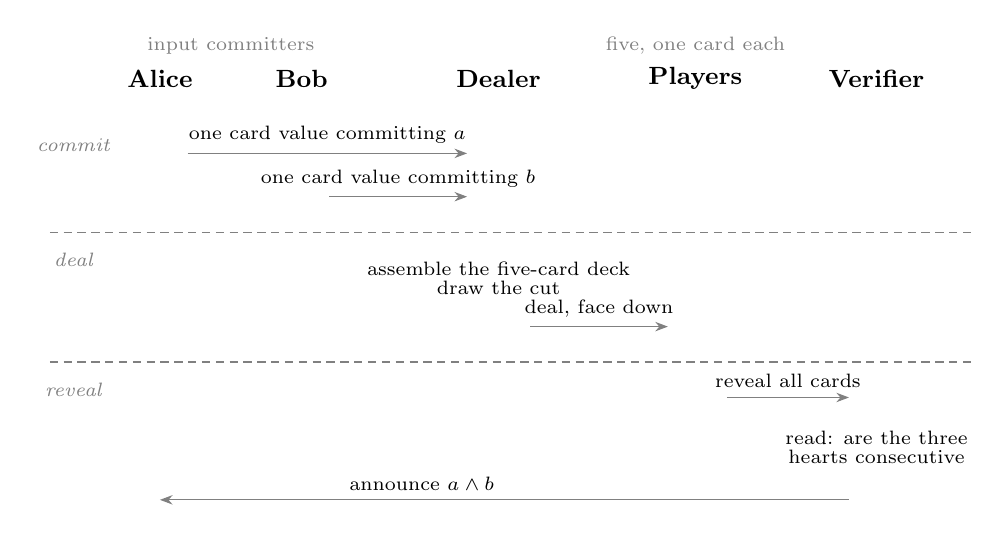
\begin{tikzpicture}[
      partyname/.style={font=\small\bfseries},
      action/.style={font=\scriptsize, align=center},
      msg/.style={-{Stealth[length=1.6mm]}, thin, draw=gray},
      lbl/.style={midway, above, font=\scriptsize},
      phase/.style={font=\scriptsize\itshape, text=gray},
      note/.style={font=\scriptsize, text=gray},
    ]
    % Party headers
    \foreach \x/\name in {1.6/Alice, 3.4/Bob, 5.9/Dealer, 8.4/Players,
                          10.7/Verifier}
      \node[partyname] at (\x, 0) {\name};
    \node[note] at (2.5, 0.42) {input committers};
    \node[note] at (8.4, 0.42) {five, one card each};

    % Phase: commit
    \node[phase] at (0.5, -0.85) {commit};
    \draw[msg] (1.95, -0.95) -- node[lbl]
      {one card value committing $a$} (5.5, -0.95);
    \draw[msg] (3.75, -1.5) -- node[lbl]
      {one card value committing $b$} (5.5, -1.5);

    % Separator
    \draw[densely dashed, gray] (0.2, -1.95) -- (11.9, -1.95);
    \node[phase] at (0.5, -2.3) {deal};

    \node[action, anchor=north] at (5.9, -2.2)
      {assemble the five-card deck\\[-1pt] draw the cut};
    \draw[msg] (6.3, -3.15) -- node[lbl] {deal, face down} (8.05, -3.15);

    % Separator
    \draw[densely dashed, gray] (0.2, -3.6) -- (11.9, -3.6);
    \node[phase] at (0.5, -3.95) {reveal};

    \draw[msg] (8.8, -4.05) -- node[lbl] {reveal all cards} (10.35, -4.05);
    \node[action, anchor=north] at (10.7, -4.35)
      {read: are the three\\[-1pt] hearts consecutive};
    \draw[msg] (10.35, -5.35) -- node[lbl, pos=0.62]
      {announce $a\wedge b$} (1.6, -5.35);
  \end{tikzpicture}
  \caption{One five-card run with committed inputs. The physical protocol
  commits each input bit as two face-down cards, and the formalization
  encodes each committed bit as one card value.}
  \label{fig:fivecard-run}
\end{figure}

\needspace{5\baselineskip}
The five-card family is the first concrete example of how the framework
components are packed into one profile. The following definition combines
the cyclic action, the biased-cut security witness, and the three-hearts
decoder.\footnote{Formalized in
\path{pgg-smc/instances/kim2025/five_card_family.v} as
\coqin{five\_card\_profile}. The listing elides the three bias
hypotheses.}

\begin{lstlisting}
Definition five_card_profile (R : realType) (eps : R)
    (* three bias hypotheses elided *) (L : nat) : MonodromyProfile R :=
  @MkMonodromyProfile R FiveCardKim_M bool FiveCardKim_PI
    (fc_kim_security_witness ... L) (* biased-cut witness    *)
    five_card_plug.                 (* three-hearts decoder  *)
\end{lstlisting}

The dealing distribution is the biased cut of Kim and \c{C}etinkaya,
and I write $w_\varepsilon$ for it:
\begin{equation}
  w_\varepsilon(a^k)=\begin{cases}\tfrac{1}{5}-\varepsilon, & k=0,\\[2pt]
  \tfrac{1}{5}+\tfrac{\varepsilon}{4}, & k=1,2,3,4,\end{cases}
  \qquad -\tfrac{4}{5}<\varepsilon<\tfrac{1}{5}.
  \label{eq:fivecard-weight}
\end{equation}
At bias zero the witness bound collapses to zero for any positive word
length. The unbiased member is therefore den Boer's protocol in
precisely this sense.\footnote{\coqin{five\_card\_eps0\_eq0} in
\path{pgg-smc/instances/kim2025/five_card_family.v}.}

What I call the master theorem gives the exact leakage for every fixed reveal set.\footnote{The master theorem \coqin{leak\_view\_set} covers all
thirty-two position subsets, anchored by \coqin{leak\_k1},
\coqin{leak\_k2\_adj}, \coqin{leak\_k2\_dist2}, \coqin{leak\_k3},
\coqin{leak\_k3\_gap}, \coqin{leak\_k4}, \coqin{leak\_k5}, and the secret's
own entropy \coqin{H\_secret} in
\path{pgg-smc/instances/denboer1989/five_card_leakage.v}. For example
\coqin{leak\_k2\_adj} $=\tfrac{27}{10}-\tfrac14\log 5-\tfrac{7}{10}\log
7$.} One revealed card carries no information about the conjunction, which
is the information-theoretic counterpart of the scheme's privacy
threshold, and the ramp climbs to the secret's own entropy
$2-\tfrac34\log 3\approx 0.811$, which I call the cap. The decimals are
evaluations of the proven closed forms.

The leakage numbers above concern the announced output. The five-card
property of the literature is input-hiding given that output: the observer
learns nothing about the input pair beyond the conjunction it announces.
The development proves this property for every reveal pattern. The input
pair and the view of any reveal set are conditionally independent given the
announced conjunction, and the corresponding conditional mutual information
is zero.\footnote{\coqin{den\_boer\_cinde} and
\coqin{den\_boer\_input\_private} in
\path{pgg-smc/instances/denboer1989/den_boer_encoding.v}, with the
reveal-set forms \coqin{cinde\_ViewS} and \coqin{input\_private\_ViewS}.}
The conditioning on the announced output is essential. The view contains
the announcement, so without the conditioning the independence fails.

Figure~\ref{fig:fivecard-leakage} selects cases that expose two features of
the leakage theorem. Two-card leakage depends on the reveal shape, while
four and five revealed cards reach the secret's entropy.

\begin{figure}[H]
  \centering
  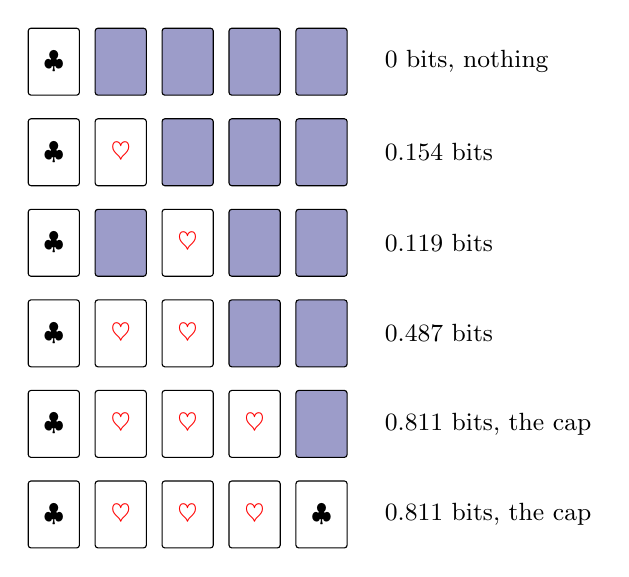
\begin{tikzpicture}[x=8.5mm,y=-11.5mm,
     card/.style={draw,rounded corners=1pt,minimum width=6.5mm,
       minimum height=8.5mm,font=\small},
     down/.style={card,fill=blue!30!gray!60},
     lab/.style={font=\small,anchor=west}]
    \node[card] at (0,1) {$\clubsuit$};
    \node[down] at (1,1) {}; \node[down] at (2,1) {};
    \node[down] at (3,1) {}; \node[down] at (4,1) {};
    \node[lab] at (4.8,1) {$0$ bits, nothing};
    \node[card] at (0,2) {$\clubsuit$};
    \node[card] at (1,2) {\textcolor{red}{$\heartsuit$}};
    \node[down] at (2,2) {}; \node[down] at (3,2) {};
    \node[down] at (4,2) {};
    \node[lab] at (4.8,2) {$0.154$ bits};
    \node[card] at (0,3) {$\clubsuit$};
    \node[down] at (1,3) {};
    \node[card] at (2,3) {\textcolor{red}{$\heartsuit$}};
    \node[down] at (3,3) {}; \node[down] at (4,3) {};
    \node[lab] at (4.8,3) {$0.119$ bits};
    \node[card] at (0,4) {$\clubsuit$};
    \node[card] at (1,4) {\textcolor{red}{$\heartsuit$}};
    \node[card] at (2,4) {\textcolor{red}{$\heartsuit$}};
    \node[down] at (3,4) {}; \node[down] at (4,4) {};
    \node[lab] at (4.8,4) {$0.487$ bits};
    \node[card] at (0,5) {$\clubsuit$};
    \node[card] at (1,5) {\textcolor{red}{$\heartsuit$}};
    \node[card] at (2,5) {\textcolor{red}{$\heartsuit$}};
    \node[card] at (3,5) {\textcolor{red}{$\heartsuit$}};
    \node[down] at (4,5) {};
    \node[lab] at (4.8,5) {$0.811$ bits, the cap};
    \node[card] at (0,6) {$\clubsuit$};
    \node[card] at (1,6) {\textcolor{red}{$\heartsuit$}};
    \node[card] at (2,6) {\textcolor{red}{$\heartsuit$}};
    \node[card] at (3,6) {\textcolor{red}{$\heartsuit$}};
    \node[card] at (4,6) {$\clubsuit$};
    \node[lab] at (4.8,6) {$0.811$ bits, the cap};
  \end{tikzpicture}
  \caption{Mutual-information leakage for selected reveal cases. Blue card
  backs mark unrevealed positions. Each value depends only on which
  positions are revealed, never on the faces drawn here, which show one
  possible outcome.}
  \label{fig:fivecard-leakage}
\end{figure}

Every three-card reveal leaks the same
$\tfrac65-\tfrac{9}{20}\log 3$ bits. The figure draws the consecutive
case, and the gapped case has the same value. Only the two-card value
depends on the pattern's shape.

\begin{example}\label{ex:fivecard-shape}
Let the reveal expose two of the five positions. Two adjacent positions
reveal $0.154$ bits about the conjunction, and two positions at cyclic
distance two reveal $0.119$ bits. Both decimals evaluate proven closed
forms, for instance the adjacent value is
$\tfrac{27}{10}-\tfrac14\log 5-\tfrac{7}{10}\log 7$. The shape stops
mattering at three revealed cards, because the closed form there depends
only on how many cards the reveal exposes.
\end{example}

The example describes what a fixed reveal set exposes. The profile also
needs a shuffle-security witness for Kim's repeated biased cut. The next
proposition supplies that witness at the concrete parameters used here.

\begin{proposition}[Seven-cut security at bias $1/100$\footnotemark]
\label{prop:fivecard-mixing}
\footnotetext{Formalized in
\path{pgg-smc/instances/kim2025/five_card_kim.v} as
\coqin{kim\_bound\_centi} and \coqin{kim\_deal\_centi\_lt}.}
Let the shuffle distribution be the biased cut $w_{1/100}$ repeated seven
times. Then every single-card endpoint distribution is within $L_1$
distance $2^{-40}$ of uniform, and the kernel checks the computation.
\end{proposition}

Because the two members share one executed program, correctness
transfers verbatim. The Kim program is the den Boer program, and its recovery
theorem is the den Boer proof reused.\footnote{\coqin{kim\_procs} and
\coqin{kim\_run\_recovers} in
\path{pgg-smc/instances/kim2025/kim_run.v}.} The committed inputs of the
two players realize the function-evaluation flow of
Section~\ref{sec:framework} with den Boer's input encoding. Den Boer's
uniform cut gives the exact endpoint distribution after one shuffle, and a
single corrupted player's executed trace leaves the secret's conditional
entropy equal to its plain
entropy.\footnote{\coqin{kim\_trace\_secrecy} in
\path{pgg-smc/instances/kim2025/kim_trace.v}.}
Table~\ref{tab:instances} in Section~\ref{sec:instances} records the full
landscape.

The five-card family keeps the group cyclic and the deck small enough for
kernel enumeration. The next sections instantiate the same records where
enumeration fails. The $\PG$ construction adds coalition privacy beyond
one card via three-transitivity, an orbit-class secret, and word
certificates proven without computing in the group.

\section{The \texorpdfstring{$\PG$}{PGL(2,7)} Construction}\label{sec:pgl}

This section constructs the paper's main eight-player instance, a model of
the profile specification: it supplies the record fields of
Section~\ref{sec:framework} and discharges their obligations. Each player
receives one card, which acts as a physical share of the secret. Under the
fixed representative dealer and an independent uniform $\PG$ shuffle, every
passive coalition of at most three players has perfect view and
executed-trace privacy. Every reveal of seven positions determines the
secret class, while every reveal of at most six positions remains compatible
with both classes. A four-position view can leak information, so the privacy
cutoff at three is sharp. The resulting recovery ramp is
$(t,r,n)=(3,7,8)$. Decoding the full eight-card arrangement is correct for
every allowed group element. Theorem~A collects these exact guarantees, and
Theorem~B later replaces the uniform group element with a uniformly sampled
200-letter generator word and bounds the resulting privacy error.

The construction indexes the eight card positions by the projective line
over $\mathbb{F}_7$:
\[
  X=\mathbb{P}^1(\mathbb{F}_7)=\{0,1,\ldots,6,\infty\}.
\]
The symbols $0,\ldots,6$ are the seven field elements, and $\infty$ is the
additional projective point. Each point labels one physical position and
therefore the player who receives the card in that position. Card values are
separate labels drawn from $C=\{0,1,\ldots,7\}$. All eight cards therefore
carry distinct symbols. This is the standard-deck setting of the card-based
literature, which caters for commonly available decks of pairwise
distinguishable cards, in contrast with the two-symbol encodings in which
most protocol sizes are measured~\cite{NiemiRenvall1999,Koch2019}. The group $G=\PG$ acts on
$X$ by fractional linear transformations. Each group element therefore
permutes the eight card positions and specifies an allowed deck
rearrangement. Its order is\footnote{Formalized in
\path{pgg-smc/instances/pgl27/pgl27_mixing.v} as \coqin{pgl27\_card}. The
order of the abstract quotient is \coqin{pgl27\_pgl2\_order} in
\path{pgg-smc/instances/pgl27/pgl27_group.v}.}
\begin{equation}
  \lvert G\rvert=336.
  \label{eq:pgl-order}
\end{equation}
The formal representation writes $\infty$ as position seven.

The $\PG$ action on $X$ induces an action on sets of four card positions.
I store the secret bit as the orbit class of the four positions occupied by
hearts. Every allowed shuffle moves this set within the same orbit, so its
orbit label remains unchanged. This invariance will give correctness under
shuffling. Privacy is a separate property of the partial observations made
by a coalition.

\subsection{Orbit Encoding of the Secret}

To make the encoding precise, we first define the reachable patterns of four
positions. We then give an explicit classifier for the two orbits, choose one
deck from each class, and prove that the classifier is unchanged by every
allowed shuffle.

\begin{definition}[Orbit of four positions]
Let
\[
  \Omega_4=\{A\subseteq X\mid |A|=4\}.
\]
For $A,B\in\Omega_4$, define
\[
  \operatorname{Orb}_G(A)=\{g\mathbin{\cdot}A\mid g\in G\},
  \qquad
  A\sim_G B
  \quad\Longleftrightarrow\quad
  B\in\operatorname{Orb}_G(A).
\]
\end{definition}

Each set $A\in\Omega_4$ records the four positions occupied by hearts without
recording which heart occupies each position. Throughout this subsection, an
orbit means an orbit in $\Omega_4$. Two heart-position patterns are
equivalent when an allowed group action carries one to the other. A valid
labelled deck therefore determines one representative of a heart-position
orbit.

To decode the orbit label from a deck, we first extract the positions
occupied by hearts. We then need an explicit test that identifies the orbit
of the resulting four-position set. The cross ratio supplies this test.

\begin{definition}[Heart-position map and decoder\footnotemark]
\footnotetext{Formalized in
\path{pgg-smc/instances/pgl27/pgl27_orbit.v} as
\coqin{is\_heart}, \coqin{deck\_ok}, \coqin{heart\_set},
\coqin{cross\_ratio}, \coqin{equianharmonic}, \coqin{subset\_class}, and
\coqin{orbit\_class}.}
A valid deck is a bijection $D:X\to C$. Its four heart values are
$0,1,2,3$, and their positions form
\[
  H(D)=\{i\in X\mid D(i)\in\{0,1,2,3\}\}\in\Omega_4.
\]
For $A=\{a<b<c<d\}$ under the order
$0<1<\cdots<6<\infty$, define the cross ratio over $\mathbb{F}_7$ by
\[
  [a,b;c,d]=\frac{(a-c)(b-d)}{(a-d)(b-c)},
  \qquad
  [a,b;c,\infty]=\frac{a-c}{b-c}.
\]
The classifier $\kappa:\Omega_4\to\{0,1\}$ is
\[
  \kappa(A)=
  \begin{cases}
    1, & [a,b;c,d]\in\{3,5\},\\
    0, & [a,b;c,d]\in\{2,4,6\}.
  \end{cases}
\]
The value one is equianharmonic, and the value zero is harmonic. The deck
decoder is
\[
  \operatorname{dec}(D)=\kappa(H(D)),
  \qquad
  D\xmapsto{H}\Omega_4\xmapsto{\kappa}\{0,1\}.
\]
\end{definition}

For $\kappa$ to serve as an orbit label, its fibers must coincide with the
orbits of $G$. Thus $\kappa$ must be constant on each orbit and must assign
different values to distinct orbits. The next theorem verifies both
requirements and counts the two fibers.

\begin{theorem}[The two orbit classes\footnotemark]
\label{thm:orbit-split}
\footnotetext{Formalized in
\path{pgg-smc/instances/pgl27/pgl27_orbit.v} as
\coqin{subset\_class\_orbit}, \coqin{subset\_class\_orbitE},
\coqin{orbit\_class\_split}, and
\coqin{orbit\_class\_split\_complement}.}
For all $A,B\in\Omega_4$,
\[
  \kappa(A)=\kappa(B)
  \quad\Longleftrightarrow\quad
  \exists g\in G,\ B=g\mathbin{\cdot}A.
\]
Hence
\[
  \Omega_4/G\cong\{0,1\},
  \qquad
  |\kappa^{-1}(0)|=42,
  \qquad
  |\kappa^{-1}(1)|=28.
\]
The fiber $\kappa^{-1}(0)$ is harmonic, and
$\kappa^{-1}(1)$ is equianharmonic.
\end{theorem}

The two orbit classes provide two stable labels and can therefore represent
the values of a Boolean secret. The dealer fixes one valid deck $D_s$ for
each label $s\in\{0,1\}$ and later distributes the shuffled cards, one to
each player. Orbit invariance will establish correctness. Privacy of the
players' partial observations is proved later from the shuffle distribution
and three-transitivity.

\begin{definition}[Orbit encoder\footnotemark]
\footnotetext{Formalized in
\path{pgg-smc/instances/pgl27/pgl27_orbit.v} as
\coqin{orbit\_encode} and \coqin{orbit\_encode\_deck}.}
The encoder chooses the valid decks
\[
  D_0=(0,1,2,3,4,5,6,7),
  \qquad
  D_1=(0,1,2,4,3,5,6,7),
\]
and sets $\operatorname{enc}(s)=D_s$.
\end{definition}

Figure~\ref{fig:encoding} shows how the two chosen decks place the four
hearts in different position patterns.

\begin{figure}[H]
  \centering
  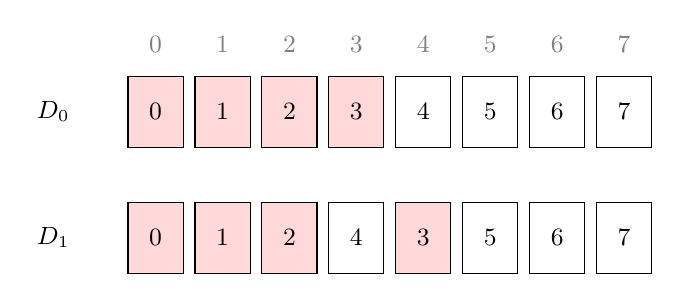
\begin{tikzpicture}[every node/.style={font=\small},
      card/.style={draw,minimum width=7mm,minimum height=9mm,inner sep=1pt},
      heart/.style={card,fill=red!15}]
    \node at (-1.3,0) {$D_0$};
    \foreach \p/\c/\s in {0/0/heart,1/1/heart,2/2/heart,3/3/heart,
                          4/4/card,5/5/card,6/6/card,7/7/card}
      \node[\s] at (\p*0.85,0) {$\c$};
    \node at (-1.3,-1.6) {$D_1$};
    \foreach \p/\c/\s in {0/0/heart,1/1/heart,2/2/heart,3/4/card,
                          4/3/heart,5/5/card,6/6/card,7/7/card}
      \node[\s] at (\p*0.85,-1.6) {$\c$};
    \foreach \p in {0,...,7}
      \node[gray] at (\p*0.85,0.85) {\p};
  \end{tikzpicture}
  \caption{The encoded representatives. Gray labels are card positions,
  with position seven representing $\infty$. Boxed numbers are card values,
  and shading marks the four heart values. The row $D_0$ represents the
  harmonic secret $0$, and $D_1$ represents the equianharmonic secret $1$.}
  \label{fig:encoding}
\end{figure}

The encoder must place each bit in the class that the decoder assigns to
that bit. The following calculation checks this round trip on both
representatives. Shuffle invariance will then extend it to every deck
reachable from either representative.

\begin{example}[Decoding the representatives\footnotemark]
\footnotetext{Formalized in
\path{pgg-smc/instances/pgl27/pgl27_orbit.v} as
\coqin{orbit\_encodeK}.}
The two rows in Figure~\ref{fig:encoding} satisfy
\[
  H(D_0)=\{0,1,2,3\},
  \qquad
  \kappa(H(D_0))=0,
\]
and
\[
  H(D_1)=\{0,1,2,4\},
  \qquad
  \kappa(H(D_1))=1.
\]
Thus the full encoding path is
\[
  s\longmapsto D_s
   \longmapsto H(D_s)
   \xmapsto{\kappa}s,
  \qquad
  \operatorname{dec}(\operatorname{enc}(s))=s.
\]
\end{example}

The example establishes
$\operatorname{dec}(\operatorname{enc}(s))=s$ before shuffling. Correctness
of a full run also requires the decoder to return the same value after every
allowed shuffle. Let $\rho:G\to S_X$ denote the induced permutation of card
positions. Since a deck $D:X\to C$ maps each position to its card value,
define
\[
  (g\star D)(i)=D(\rho(g)(i)).
\]
The symbol $\star$ denotes this rearrangement of decks. Position $i$ in
$g\star D$ holds the value from position $\rho(g)(i)$ in $D$. The following
lemma tracks how this convention moves the heart positions.

\begin{lemma}[Shuffle invariance\footnotemark]
\footnotetext{Formalized in
\path{pgg-smc/instances/pgl27/pgl27_orbit.v} as
\coqin{subset\_class\_invariant}, \coqin{orbit\_class\_invariant}, and
\coqin{deck\_stable}. The heart-set identity is the local equality
\coqin{Hheart} in the proof of \coqin{orbit\_class\_invariant}, not a
separate exported theorem.}
For every $g\in G$ and valid deck $D$,
\[
  H(g\star D)=\rho(g)^{-1}\mathbin{\cdot}H(D).
\]
The shuffled deck also satisfies
\[
  g\star D\text{ is valid},
  \qquad
  \operatorname{dec}(g\star D)=\operatorname{dec}(D).
\]
\end{lemma}

Because $\rho(g)^{-1}=\rho(g^{-1})$, the heart set of the shuffled deck
remains in the same $G$-orbit as $H(D)$. The shuffle may change the
representative in $\Omega_4$, but it cannot change the orbit label.

In one run, the dealer encodes $s$ as $D_s$, applies an allowed shuffle, and
distributes one card to each player. When all eight players reveal their
cards, the verifier sees $g\star D_s$. The following corollary gives the
deck-level correctness required by this execution. Proposition~\ref{thm:pgl-correctness}
later lifts this equality to the executable interpreter. The recovery
threshold and coalition privacy are separate properties proved in
Section~\ref{sec:exact}.

\begin{corollary}[Shuffle correctness of orbit decoding\footnotemark]
\label{cor:orbit-shuffle-correctness}
\footnotetext{The direct equality is formalized in
\path{pgg-smc/instances/pgl27/pgl27_orbit.v} as
\coqin{orbit\_encodeK} and \coqin{orbit\_class\_invariant}. The
reconstruction-interface counterpart is
\coqin{orbit\_recon\_invariant} in
\path{pgg-smc/instances/pgl27/pgl27_scheme.v}.}
For every $s\in\{0,1\}$ and $g\in G$,
\[
  \operatorname{dec}(g\star\operatorname{enc}(s))
  =\operatorname{dec}(\operatorname{enc}(s))
  =s.
\]
\end{corollary}

By Corollary~\ref{cor:orbit-shuffle-correctness}, every allowed shuffle
preserves the decoded secret of an encoded deck. This correctness result
does not imply privacy. When $g\leftarrow U_G$ is independent of the secret,
privacy is a property of the distribution of partial observations. The
privacy proof uses three-transitivity as its group-action premise.

Figure~\ref{fig:run} shows how the encoder and decoder enter one execution.

\begin{figure}[H]
  \centering
  % Drawn at true document font sizes; the picture is never scaled.
  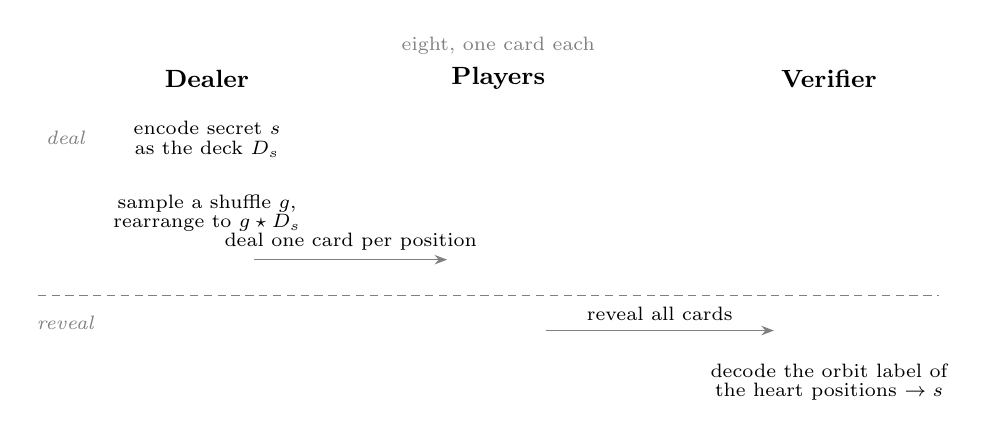
\begin{tikzpicture}[
      partyname/.style={font=\small\bfseries},
      action/.style={font=\scriptsize, align=center},
      msg/.style={-{Stealth[length=1.6mm]}, thin, draw=gray},
      lbl/.style={midway, above, font=\scriptsize},
      phase/.style={font=\scriptsize\itshape, text=gray},
      note/.style={font=\scriptsize, text=gray},
    ]
    % Party headers
    \foreach \x/\name in {2.3/Dealer, 6.0/Players, 10.2/Verifier}
      \node[partyname] at (\x, 0) {\name};
    \node[note] at (6.0, 0.42) {eight, one card each};

    % Phase: deal
    \node[phase] at (0.5, -0.75) {deal};
    \node[action, anchor=north] at (2.3, -0.42)
      {encode secret $s$\\[-1pt] as the deck $D_s$};
    \node[action, anchor=north] at (2.3, -1.35)
      {sample a shuffle $g$,\\[-1pt] rearrange to $g\star D_s$};
    \draw[msg] (2.9, -2.3) -- node[lbl]
      {deal one card per position} (5.35, -2.3);

    % Separator
    \draw[densely dashed, gray] (0.15, -2.75) -- (11.6, -2.75);
    \node[phase] at (0.5, -3.1) {reveal};

    \draw[msg] (6.6, -3.2) -- node[lbl] {reveal all cards} (9.5, -3.2);
    \node[action, anchor=north] at (10.2, -3.5)
      {decode the orbit label of\\[-1pt] the heart positions $\to s$};
  \end{tikzpicture}
  \caption{One $\PG$ run: eight players, one card each, no player inputs,
  and the verifier decodes the orbit label of the heart positions. The
  shuffle $g$ is drawn from the uniform distribution $U_G$ in the
  uniform-shuffle model and from the word distribution $\worddist$ in the
  word-shuffle model. This is the no-input counterpart of
  Figure~\ref{fig:fivecard-run}.}
  \label{fig:run}
\end{figure}

\subsection{Action and Generators}

The protocol uses the permutation action $\rho:G\to S_X$ on the eight card
positions. A generator is one of a fixed set of group elements whose finite
products reach every element of $G$. Under $\rho$, each generator specifies
a rearrangement of the eight cards. A generator word specifies a
sequence of these rearrangements. In the passive execution model, no party
records the intermediate arrangements, so the word enters the execution
only through its product $g\in G$ and the resulting deck $g\star D_s$.

For $G=\PG$, three fractional linear maps generate the group. They are the
translation $z\mapsto z+1$, the scaling $z\mapsto 3z$, and the inversion
$z\mapsto -1/z$.\footnote{The rows of Figure~\ref{fig:pgl-generators} are
the permutation tables of the three maps, identified with them by
\coqin{tr\_moebius}, \coqin{sc\_moebius}, and \coqin{inv\_moebius} in
\path{pgg-smc/instances/pgl27/pgl27_group.v}.}
Figure~\ref{fig:pgl-generators} shows each generator as a rearrangement of
the row of eight cards, one card per projective point. The five-letter
alphabet of the executable shuffle in Section~\ref{sec:mixing} contains
these three maps together with the inverses of translation and scaling.
The equality $|G|=336=8\cdot7\cdot6$ also matches the number of ordered
triples of distinct points. Lemma~\ref{thm:three-transitive} produces a
group element for each ordered destination, and the count equality makes
that element unique.

\begin{figure}[t]
  \centering
  % Drawn at true document font sizes; the picture is never scaled.
  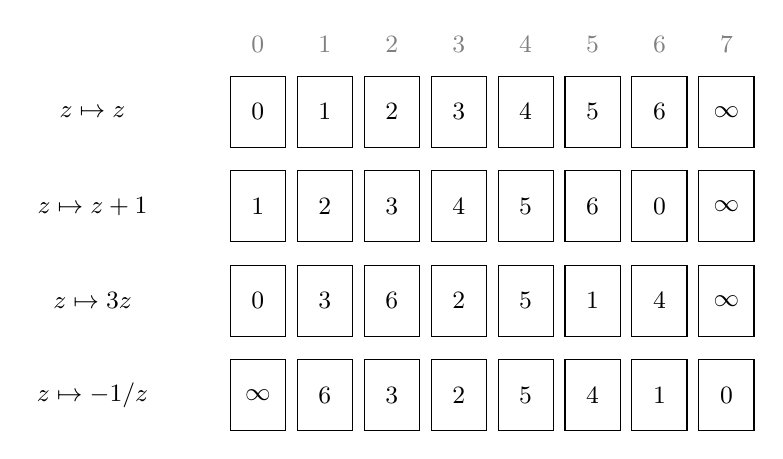
\begin{tikzpicture}[every node/.style={font=\small},
      card/.style={draw,minimum width=7mm,minimum height=9mm,inner sep=1pt}]
    \foreach \p in {0,...,7}
      \node[gray] at (\p*0.85,0.85) {\p};
    \node at (-2.1,0) {$z\mapsto z$};
    \foreach \p/\c in {0/0,1/1,2/2,3/3,4/4,5/5,6/6,7/\infty}
      \node[card] at (\p*0.85,0) {$\c$};
    \node at (-2.1,-1.2) {$z\mapsto z+1$};
    \foreach \p/\c in {0/1,1/2,2/3,3/4,4/5,5/6,6/0,7/\infty}
      \node[card] at (\p*0.85,-1.2) {$\c$};
    \node at (-2.1,-2.4) {$z\mapsto 3z$};
    \foreach \p/\c in {0/0,1/3,2/6,3/2,4/5,5/1,6/4,7/\infty}
      \node[card] at (\p*0.85,-2.4) {$\c$};
    \node at (-2.1,-3.6) {$z\mapsto -1/z$};
    \foreach \p/\c in {0/\infty,1/6,2/3,3/2,4/5,5/4,6/1,7/0}
      \node[card] at (\p*0.85,-3.6) {$\c$};
  \end{tikzpicture}
  \caption{The three generating maps on the projective points. Gray labels
  are positions, and the box at position $i$ shows the image point $g(i)$.
  The symbol $\infty$ is position seven.}
  \label{fig:pgl-generators}
\end{figure}

The figure gives the three permutation tables. The following example reads
them as physical row movements and connects words in these generators to
the triple transport used below.

\begin{example}\label{ex:pgl-letters}
Use projective-point labels to display the identity assignment, with label
$z$ at position $z$.
The translation map turns the row $(0,1,2,3,4,5,6,\infty)$ into
$(1,2,3,4,5,6,0,\infty)$ because position $i$ shows the image $g(i)$.
The scaling map fixes $0$ and $\infty$ and moves the six remaining
points in one six-cycle. The inversion map is an involution. It
exchanges $0$ with $\infty$, $1$ with $6$, $2$ with $3$, and $4$ with
$5$. Words in the three maps reach every one of the $336$ group
elements.
Lemma~\ref{thm:three-transitive} below gives one such word for every
ordered triple of distinct points. For example, the five-letter word that
applies the inverse scaling, then the inverse translation, then the
inversion, then the scaling, and then the inverse translation evaluates to
the map $z\mapsto(z-1)/(3-z)$, which carries $(0,1,2)$ to $(2,0,1)$.
\end{example}

\subsection{Three-Transitivity and Local Views}

The organizing fact of this instance is that the action of $\PG$ on the
eight projective points is sharply three-transitive. Any ordered triple of
distinct points is carried to any other by exactly one group element,
because the order $336=8\cdot7\cdot6$ equals the number of ordered triples.
Under a uniform shuffle, three revealed positions therefore carry no
invariant at all, and four positions carry exactly one, the cross ratio.
This single fact organizes the instance: it makes the cross-ratio decoder
exist, caps perfect privacy at coalitions of size three, forces
four-position coalitions to leak, and is the reason the construction uses
$\PG$.

Global orbit invariance gives correctness. Privacy asks a different question:
what does a small named set of positions observe when $g\leftarrow U_G$ is
independent and uniform? Ordered tuples matter because a coalition observes
card values at named positions.

\vfill\pagebreak
\begin{lemma}[Three-transitivity\footnotemark]\label{thm:three-transitive}
\footnotetext{Formalized in \path{pgg-smc/instances/pgl27/pgl27_group.v} as
\coqin{pgl27\_3transitive}.}
For any ordered triples $(x_1,x_2,x_3)$ and $(y_1,y_2,y_3)$ of distinct
projective points, there is a $g\in\PG$ such that
\[
  g(x_1)=y_1, \qquad g(x_2)=y_2, \qquad g(x_3)=y_3.
\]
\end{lemma}

The formal proof enumerates generator words that send a fixed base triple to
each distinct target triple. The kernel checks the resulting finite table. For example, the base
triple is $(0,1,2)$, and the table stores for every other ordered triple
of distinct points one generator word that carries $(0,1,2)$ to it.
Lemma~\ref{thm:three-transitive} makes every ordered view of at most three
positions uniform under $U_G$. It supplies the group-action premise of
Theorem~\ref{thm:generic-privacy} at $t=3$. That theorem then gives
uniform-shuffle coalition privacy. The nonuniform word distribution is treated
separately in Section~\ref{sec:mixing}.

Table~\ref{tab:source-index} at the end of Section~\ref{sec:mixing}
indexes the formal sources for this section and the two that follow.

\section{Correctness, Recovery, and Uniform-Shuffle Privacy}\label{sec:exact}

The construction section established deck-level correctness and the
group-action premise for privacy. This section lifts correctness to the
executed protocol, determines the recovery ramp, and proves view and trace
privacy under a uniform shuffle. These results form Theorem A.

\subsection{Correctness and Recovery}

The interpreter deals $D_s$, applies an allowed shuffle, and sends one card
to each of eight players.\footnote{The dealer program is
\coqin{exchange\_dealer} and the $\PG$ witness is the singleton cut list in
\coqin{pgl27\_dealer\_run}.} The players return their cards to the verifier. The
verifier's endpoint sequence is the shuffled dealt arrangement. Orbit-class
invariance and the encoder equation then give correctness.

\begin{proposition}[Executed correctness\footnotemark]\label{thm:pgl-correctness}
\footnotetext{Formalized in \path{pgg-smc/instances/pgl27/pgl27_run.v} as
\coqin{pgl27\_run\_recovers}. The direct class-recovery counterpart is
formalized in \path{pgg-smc/instances/pgl27/pgl27_trace.v} as
\coqin{pgl27\_run\_recovers\_class}.}
\par
For every $s\in\{0,1\}$ and $g\in\PG$, decoding all eight verifier endpoints
after the shuffle $g$ returns $s$.
\end{proposition}

Correctness quantifies over every group element. It therefore holds with
probability one under the uniform distribution and under any word distribution, and only
privacy carries an approximation error. A corollary instantiates the
executed run at the evaluated 200-letter word.\footnote{The corollary is
\coqin{pgl27\_word\_run\_recovers} in
\path{pgg-smc/instances/pgl27/pgl27_word_privacy.v}.}

Recovery has a finer threshold than the implemented decoder exposes. Any
seven revealed positions determine the missing card because a valid deck uses
all eight card values once. Hence seven revealed positions determine the
orbit class. By contrast, every set of at most six revealed positions is
consistent with valid arrangements from both secret classes.

Three parameters summarize the instance, and the two thresholds live on
different axes. The privacy threshold $t$ is defined as the largest
coalition size with perfect privacy, a probabilistic condition: the
coalition's view is independent of the secret. The recovery threshold $r$
is defined as the least number of revealed positions that always
determines the secret class, a possibilistic condition: below it, both
classes remain consistent with the revealed cards. The number of card
positions is $n$. I call the triple $(t,r,n)$ the recovery ramp, following
the ramp schemes of the secret-sharing literature, in which the gap between
the two thresholds is the graded regime between privacy and
recovery~\cite{BlakleyMeadows1984,Yamamoto1986}. The implemented decoder
reads all eight endpoints, so $r=7$ is a structural threshold of the
arrangement combinatorics rather than the reading rule of a smaller
implemented decoder.

\begin{proposition}[Recovery ramp and sharpness\footnotemark]\label{thm:recovery-ramp}
\footnotetext{Formalized in \path{pgg-smc/instances/pgl27/pgl27_recovery.v}
as \coqin{pgl27\_reveal\_ambiguous} and
\coqin{pgl27\_seven\_reveal\_class}, and in
\path{pgg-smc/instances/pgl27/pgl27_secrecy.v} as
\coqin{pgl27\_view\_dep\_k4} and \coqin{pgl27\_view\_leak\_k4}.}
Every reveal set of at most six positions is compatible with valid
arrangements from both secret classes, and every set of seven revealed
positions determines the secret class. The view of the coalition of the
four heart positions in the identity arrangement depends on the secret and
has positive mutual information with it.
\end{proposition}

The recovery result and the privacy result have different cutoffs. Perfect
coalition privacy holds through size three, while deterministic recovery
begins at size seven. Figure~\ref{fig:ramp} places them on separate tracks.

\begin{figure}[t]
  \centering
  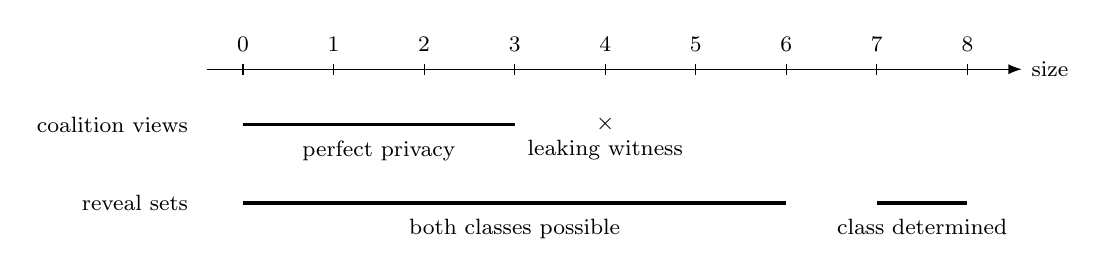
\begin{tikzpicture}[every node/.style={font=\footnotesize},xscale=1.15]
    \draw[-{Latex}] (-0.4,0) -- (8.6,0) node[right] {size};
    \foreach \x in {0,...,8}
      \draw (\x,-0.07) -- (\x,0.07) node[above=1pt] {\x};
    \node[left] at (-0.5,-0.7) {coalition views};
    \draw[very thick] (0,-0.7) -- (3,-0.7)
      node[midway,below=2pt] {perfect privacy};
    \node at (4,-0.7) {$\times$};
    \node[below=2pt] at (4,-0.7) {leaking witness};
    \node[left] at (-0.5,-1.7) {reveal sets};
    \draw[very thick] (0,-1.7) -- (6,-1.7)
      node[midway,below=2pt] {both classes possible};
    \draw[very thick] (7,-1.7) -- (8,-1.7)
      node[midway,below=2pt] {class determined};
  \end{tikzpicture}
  \caption{The recovery ramp $(t,r,n)=(3,7,8)$. The view track shows
  perfect privacy for coalitions of at most three positions and the leaking
  four-position witness. The reveal track shows ambiguity through six
  positions and determination from seven.}
  \label{fig:ramp}
\end{figure}

The witness coalition
makes the privacy cutoff three sharp. The leakage for reveal sets of sizes
four through six reduces to four numbers, one per orbit of reveal sets
under $G$. The four-subsets fall into two orbits, of sizes $42$ and $28$,
separated by the classical cross-ratio invariant, and the five-subsets and
the six-subsets each form a single orbit.\footnote{The orbit census and the collision counts are kernel-checked
in \path{pgg-smc/instances/pgl27/pgl27_leakage_census.v}, as
\coqin{pgl27\_orbit\_four\_cover}, \coqin{pgl27\_five\_subset\_orbitE},
\coqin{pgl27\_six\_subset\_orbitE}, and the \coqin{pgl27\_collisions}
lemmas.} For a representative $C$ with at least three positions, the two
deals restrict to $C$ injectively, so, given either secret value, the
coalition's observation is uniform over the $336$ equally likely
possibilities, and the mutual information between the secret class
and the revealed cards equals $1-m/336$ bits, where $m$ counts the
observations shared by the two deals. This identity is a pen-and-paper step
justified by sharp three-transitivity, and it fails below three positions,
where the true leakage is zero. The kernel-checked collision counts of the
four representatives are $m=96$, $72$, $36$, and $12$, so the leakage
values are $5/7$, $11/14$, $25/28$, and $27/28$ bits, evaluated from the
counts outside the kernel by the committed script
\path{pgg-smc/instances/pgl27/pgl_leakage_targets.py}. The four-heart
witness coalition is the representative of the $42$-element orbit, and its
leakage is exactly $5/7$ bits. Extending each number from its
representative to the whole orbit uses invariance of leakage under
relabeling by a group element, a pen-and-paper step that the development
does not formalize.

\subsection{Perfect View and Trace Privacy}

The main uniform-shuffle execution samples $S$ uniformly from $\{0,1\}$. It deals the
fixed representative $D_S$ and samples an independent shuffle $g\leftarrow
U_G$.\footnote{The execution distribution is \coqin{pgl27P} and the
representative is the formal orbit encoder \coqin{orbit\_encode}.} Three-transitivity gives independence for every coalition $C$ with
$\lvert C\rvert\leq3$.

\begin{proposition}[Perfect privacy for the fixed dealer\footnotemark]
\footnotetext{Formalized in \path{pgg-smc/instances/pgl27/pgl27_secrecy.v}
as
\coqin{pgl27\_view\_indep}. The trace counterpart is formalized in
\path{pgg-smc/instances/pgl27/pgl27_trace.v} as
\coqin{pgl27\_coalition\_trace\_secrecy}.}
Under the uniform Boolean prior, the fixed representative dealer, and an
independent uniform $\PG$ shuffle,
\[
  S\mathrel{\perp}V_C
  \quad\text{and}\quad
  H(S\mid T_C)=H(S)
  \qquad\text{for every }\lvert C\rvert\leq3.
\]
\end{proposition}

\begin{example}\label{ex:coalition-view}
Let the dealt secret be $s=0$, so the dealt arrangement is $D_0$, and let
the shuffle be the translation $x\mapsto x+1$, which fixes the point
$\infty$ at position seven. Each position then shows the card that $D_0$
places one position later, and the coalition $\{0,1,2\}$ sees the card
values $(1,2,3)$. At $s=1$ the same shuffle would show $(1,2,4)$. By
Lemma~\ref{thm:three-transitive} some shuffle instead sends the
coalition's three positions to the positions $1$, $2$, and $4$ of $D_1$,
which hold the values $1$, $2$, and $3$. A coalition of three cards
therefore never separates the two secrets, and the proposition above makes
this uniformity exact.
\end{example}

Two further dealers act as robustness checks on the fixed representative.
The all-decks dealer tests whether the fixed representative hides a special
choice. It samples $S$ uniformly. Conditional on $S=s$, it samples a uniform
valid arrangement of class $s$. It then applies an independent uniform
$\PG$ shuffle.\footnote{The all-decks distribution is
\coqin{pgl27P\_alldecks}.}

\begin{proposition}[All-decks perfect privacy\footnotemark]
\footnotetext{Formalized in \path{pgg-smc/instances/pgl27/pgl27_secrecy.v}
as
\coqin{pgl27\_view\_indep\_alldecks}. The trace counterpart is formalized in
\path{pgg-smc/instances/pgl27/pgl27_trace.v} as
\coqin{pgl27\_alldecks\_coalition\_secrecy}.}
Under the uniform Boolean prior, the uniform class-conditional deck dealer,
and an independent uniform $\PG$ shuffle,
\[
  S\mathrel{\perp}V_C
  \quad\text{and}\quad
  H(S\mid T_C)=H(S)
  \qquad\text{for every }\lvert C\rvert\leq3.
\]
\end{proposition}

A third dealer samples a uniform valid deck in the chosen class and applies
no later shuffle. I call the resulting distribution the shuffle-free deck
distribution, and view independence holds under it for
every Boolean secret prior. The available executed-trace theorem uses the
uniform Boolean prior. No prior-generic trace theorem is claimed.

\begin{proposition}[Shuffle-free deck privacy\footnotemark]
\footnotetext{Formalized in \path{pgg-smc/instances/pgl27/pgl27_secrecy.v}
as
\coqin{pgl27\_view\_indep\_deck\_prior}. The trace counterpart is formalized
in \path{pgg-smc/instances/pgl27/pgl27_trace.v} as
\coqin{pgl27\_deck\_coalition\_secrecy}.}
For any Boolean prior, the uniform class-conditional deck gives
$S\mathrel{\perp}V_C$ whenever $\lvert C\rvert\leq3$. Under the uniform
Boolean prior, it also gives $H(S\mid T_C)=H(S)$.
\end{proposition}

Executed correctness supplies full-run decoding. The recovery-ramp
proposition supplies the recovery threshold and the four-card leakage
witness. Fixed-dealer privacy supplies view and trace privacy through size
three, which makes the four-card witness sharp. Together these results give
the first headline theorem.

\begin{thmA}
The $\PG$ instance recovers the secret from all eight endpoints for every
group element.\footnotemark{} Under the uniform Boolean prior, the fixed
representative dealer, and an independent uniform $\PG$ shuffle, the
instance has recovery parameters
\[
  (t,r,n)=(3,7,8),
\]
and for every passive coalition $C$ with $\lvert C\rvert\leq3$,
\[
  S\mathrel{\perp}V_C
  \quad\text{and}\quad
  H(S\mid T_C)=H(S).
\]
\end{thmA}
\footnotetext{This statement is the conjunction of the following formalized
results: \coqin{pgl27\_run\_recovers} in
\path{pgg-smc/instances/pgl27/pgl27_run.v}, \coqin{pgl27\_reveal\_ambiguous}
and \coqin{pgl27\_seven\_reveal\_class} in
\path{pgg-smc/instances/pgl27/pgl27_recovery.v},
\coqin{pgl27\_view\_leak\_k4} and \coqin{pgl27\_view\_indep} in
\path{pgg-smc/instances/pgl27/pgl27_secrecy.v}, and
\coqin{pgl27\_coalition\_trace\_secrecy} in
\path{pgg-smc/instances/pgl27/pgl27_trace.v}.}

The trust base for these results is stated in
Section~\ref{sec:instances}.

Theorem A uses a uniform group element. The next section replaces this
ideal shuffle with a finite generator word and bounds the resulting error.

\section{Word-Shuffle Approximation of the Uniform-Shuffle Model}\label{sec:mixing}

Section~\ref{sec:model} defines the generator word. This section proves a
machine-checked mixing certificate for the finitely generated shuffle: the
evaluated distribution of a uniform word is close to the uniform
distribution on the group. The letters are group generators rather than
cuts of the eight-card row, and I do not claim a physical realization of an
unobserved letter application. The certificate is the object of interest,
since it bounds the distance of the executable shuffle from the ideal one.
The proof transfers this bound to the security observables, and Theorem B
gives the final bound.

The executable shuffle samples a word over five letters. Three letters are
the projective translation, scaling, and inversion generators. The alphabet
also contains the inverses of translation and scaling. Inversion is already
self-inverse. The alphabet includes the two inverse letters because the fiber
computation below steps backward through a letter's inverse and must stay
inside the alphabet. The symmetric tuple still generates the same group
as the original three generators, so the fiber count concerns the same
$336$ elements.

For a word length $L$, the shuffle distribution evaluates a uniform word in
$\{0,1,2,3,4\}^L$. For instance, at the Theorem B length $L=200$ the sample space contains
$5^{200}$ words.
The proof partitions these words by evaluated group element. I call the
set of words that evaluate to $g$ the fiber of $g$, and there are $336$
fibers. Roughly speaking, the certificate counts how often each of the
$336$ group elements occurs among the $5^{200}$ words and checks that no
element occurs much more or much less often than average. For example, at $L=1$ the word consisting of the translation letter
evaluates to $z\mapsto z+1$ and belongs to the fiber of that group element.
A computation over binary naturals records the size of every
fiber. The final arithmetic check sums the deviations of these fiber counts
from $5^{200}/336$.

\begin{lemma}[Word-shuffle mixing bound\footnotemark]\label{thm:pgl-mixing}
\footnotetext{Formalized in \path{pgg-smc/instances/pgl27/pgl27_mixing.v} as
\coqin{pgl27\_word\_mixing}.}
Let $\mu$ be uniform on the five-letter symmetric generator tuple. Then
\begin{equation}
  \left\lVert \mu^{*200}-U_G\right\rVert_1 \leq 2^{-40}.
  \label{eq:pgl-mixing}
\end{equation}
\end{lemma}

Equation~\ref{eq:pgl-mixing} is one checked certificate, which I call
the mixing certificate. Its inputs are the
five-letter generation theorem, the group order in
Equation~\ref{eq:pgl-order}, the $336$ fiber counts, and the final integer
inequality. The certificate concerns the distribution of shuffle group
elements.

A coalition observes card endpoints rather than group elements. The
certificate therefore moves from the group to the endpoints first. The
first transfer, which I call the endpoint transfer, maps each
permutation to the endpoint of one fixed card.

\begin{lemma}[Endpoint transfer\footnotemark]\label{lem:endpoint-transfer}
\footnotetext{Formalized in \path{pgg-smc/instances/pgl27/pgl27_mixing.v}
as \coqin{pgl27\_endpoint\_mixing}.}
By the $L_1$ data-processing inequality, for every card position $i$,
\begin{equation}
  \left\lVert
    (g\mapsto \rho(g)i)_\#\mu^{*200}
    -(g\mapsto \rho(g)i)_\#U_G
  \right\rVert_1
  \leq 2^{-40}.
  \label{eq:endpoint-transfer}
\end{equation}
\end{lemma}

The endpoint transfer controls one card position, and transitivity makes
its uniform-shuffle endpoint distribution uniform on the eight positions.
The privacy theorem also tracks the secret. The next lemma takes the product
of both shuffle distributions with the same independent Boolean prior and
preserves the $L_1$ bound.

\begin{lemma}[Secret-prior product transfer\footnotemark]\label{lem:product-transfer}
\footnotetext{Formalized in \path{pgg-smc/instances/pgl27/pgl27_mixing.v}
as \coqin{pgl27\_joint\_mixing}.}
Let $\pi$ be any distribution on Boolean secrets. Independence is built
into the product distributions, and
\begin{equation}
  \left\lVert
    \pi\mathbin{\times}\mu^{*200}
    -\pi\mathbin{\times}U_G
  \right\rVert_1
  \leq 2^{-40}.
  \label{eq:product-transfer}
\end{equation}
\end{lemma}

Equations~\ref{eq:endpoint-transfer} and~\ref{eq:product-transfer}
transfer the one certificate of Equation~\ref{eq:pgl-mixing} to two
further sample spaces. Neither is a separate mixing certificate, and
Equation~\ref{eq:product-transfer} still compares a prior with a shuffle
distribution rather than a distribution over executed runs.

The proved chain reaches group-distribution proximity, every single-card
marginal, and the product with any secret prior. Transport through the
protocol interpreter turns the certificate into the second headline
theorem.

\begin{thmB}
Let $\mu$ be uniform on the five-letter symmetric generator
tuple.\footnotemark{} Then
\[
  \left\lVert \mu^{*200}-U_G\right\rVert_1 \leq 2^{-40}.
\]
For the fixed representative dealer, every passive coalition $C$ with
$\lvert C\rvert\leq3$, and all secrets $s,s'\in\{0,1\}$, where the coalition
view at dealt secret $s$ and shuffle $g$ is denoted $V_C(s,g)$,
\begin{equation}
  \left\lVert
    (g\mapsto V_C(s,g))_\#\mu^{*200}
    -(g\mapsto V_C(s',g))_\#\mu^{*200}
  \right\rVert_1
  \leq 2^{-39},
  \label{eq:word-view-privacy}
\end{equation}
and the executed coalition trace satisfies the same bound. Decoding all
eight endpoints returns the dealt secret for every word.
\end{thmB}
\footnotetext{This statement is the conjunction of the following formalized
results: \coqin{pgl27\_word\_mixing} in
\path{pgg-smc/instances/pgl27/pgl27_mixing.v}, and
\coqin{pgl27\_word\_view\_indist}, \coqin{pgl27\_word\_trace\_indist}, and
\coqin{pgl27\_word\_run\_recovers} in
\path{pgg-smc/instances/pgl27/pgl27_word_privacy.v}.}

The proof is a triangle inequality through the uniform group distribution. The
coalition-view distribution under the uniform shuffle does not depend on the secret,
by three-transitivity. The data-processing inequality applies the
certificate in Equation~\ref{eq:pgl-mixing} on each side of the triangle. A
companion theorem bounds the joint view-and-secret distribution under the word
shuffle against the product of its uniform-shuffle marginals by $2^{-40}$ at
any Boolean prior.\footnote{The companion result is
\coqin{pgl27\_view\_mixing}. It is an ideal-proximity statement, not the
privacy definition.}

The word-shuffle privacy results cover the fixed representative dealer only,
since the all-decks and shuffle-free dealers use different sample spaces
that the product-distribution transfer does not reach. The trust base for
these results is stated in Section~\ref{sec:instances}.

The PGL argument has four proof layers: construction, recovery, privacy,
and finite-word transfer. Table~\ref{tab:source-index} maps the
mathematical claims used by Theorems A and B to the \Rocq{} results that
establish them.

\begin{table}[H]
  \centering
  \small
  \begin{tabular}{p{.40\linewidth}p{.50\linewidth}}
    \toprule
    Mathematical statement & Rocq source name \\
    \midrule
    \multicolumn{2}{@{}l}{\emph{Construction}} \\
    three-transitivity & \coqin{pgl27\_3transitive} \\
    equianharmonic and harmonic counts & \coqin{orbit\_class\_split},
      \coqin{orbit\_class\_split\_complement} \\
    encoder returns its class & \coqin{orbit\_encodeK} \\
    group order & \coqin{pgl27\_card} \\
    \midrule
    \multicolumn{2}{@{}l}{\emph{Correctness and recovery}} \\
    executed class recovery & \coqin{pgl27\_run\_recovers\_class} \\
    seven cards determine deck and class &
      \coqin{pgl27\_seven\_reveal\_determines},
      \coqin{pgl27\_seven\_reveal\_class} \\
    at most six cards remain ambiguous &
      \coqin{pgl27\_six\_reveal\_ambiguous},
      \coqin{pgl27\_reveal\_ambiguous} \\
    four-card dependence and leakage &
      \coqin{pgl27\_view\_dep\_k4}, \coqin{pgl27\_view\_leak\_k4} \\
    \midrule
    \multicolumn{2}{@{}l}{\emph{Privacy}} \\
    fixed representative views &
      \coqin{pgl27\_view\_indep}, \coqin{pgl27\_view\_leakage\_le} \\
    fixed representative traces &
      \coqin{pgl27\_trace\_secrecy},
      \coqin{pgl27\_coalition\_trace\_secrecy} \\
    all-decks views and traces &
      \coqin{pgl27\_view\_indep\_alldecks},
      \coqin{pgl27\_alldecks\_trace\_secrecy},
      \coqin{pgl27\_alldecks\_coalition\_secrecy} \\
    shuffle-free views and traces &
      \coqin{pgl27\_view\_indep\_deck\_prior},
      \coqin{pgl27\_deck\_trace\_secrecy},
      \coqin{pgl27\_deck\_coalition\_secrecy} \\
    \midrule
    \multicolumn{2}{@{}l}{\emph{Mixing and transfers}} \\
    word mixing certificate & \coqin{pgl27\_word\_mixing} \\
    endpoint and product transfers &
      \coqin{pgl27\_endpoint\_mixing}, \coqin{pgl27\_joint\_mixing} \\
    word view and trace bounds &
      \coqin{pgl27\_word\_view\_indist},
      \coqin{pgl27\_word\_trace\_indist} \\
    ideal-proximity companion & \coqin{pgl27\_view\_mixing} \\
    word correctness & \coqin{pgl27\_word\_run\_recovers} \\
    \bottomrule
  \end{tabular}
  \caption{Rocq sources for the $\PG$ results.}
  \label{tab:source-index}
\end{table}

\section{Other Instances and Trust Base}\label{sec:instances}

The framework's value shows in which arguments transfer across instances
unchanged and which need instance-specific finite or spectral evidence.
Beyond the instances of Sections~\ref{sec:fivecard} and~\ref{sec:pgl}, the
$S_5$ and $S_5\times S_5$ instances exercise the spectral part of the
framework, and Table~\ref{tab:instances} records the proved coverage
across all five. For example, the trace-lifting theorem of
Section~\ref{sec:framework} is consumed verbatim by all five instances,
while each instance supplies its own endpoint bound. Perfect privacy in
the table refers to the dealer distribution defined by each
instance.
The trace column records no second security property: it records the
interpreter-soundness transport of the same view privacy to the executed
trace of the stated corrupted players.

The PGL instance adds coalition views, coalition traces, the recovery ramp,
and the finite fiber certificate from Section~\ref{sec:mixing}. Its mixing
result does not depend on the $S_5$ Rayleigh premise.

\begin{table}[t]
  \centering
  \small
  \renewcommand{\arraystretch}{1.15}
  \begin{tabular}{@{}L{.14\linewidth}L{.24\linewidth}
                       L{.25\linewidth}L{.22\linewidth}@{}}
    \toprule
    Instance & Recovery & Perfect privacy & Trace transport \\
    \midrule
    den Boer & five-card AND & one card & one player \\
    Kim & five-card AND & one card & one player \\
    $S_5$ & additive 5-of-5 & fewer than five & one player \\
    $S_5\times S_5$ & two additive 5-of-5 shares
      & fewer than five per pile & one player \\
    $\PG$ & $(t,r,n)=(3,7,8)$ & coalitions of at most three
      & coalitions of at most three \\
    \bottomrule
  \end{tabular}

  \vspace{1ex}

  \begin{tabular}{@{}L{.14\linewidth}L{.40\linewidth}L{.31\linewidth}@{}}
    \toprule
    Instance & Word-shuffle mixing & Trust base \\
    \midrule
    den Boer & exact after one uniform cut & kernel, \coqin{boolp} \\
    Kim & $L=7$, $L_1<2^{-40}$ & kernel, \coqin{boolp} \\
    $S_5$ & $L=286$ spectral route & imported Rayleigh bound \\
    $S_5\times S_5$ & within-pile decay, global floor $1$
      & inherited Rayleigh bound \\
    $\PG$ & $L=200$, $L_1\leq2^{-40}$ & kernel, \coqin{boolp} \\
    \bottomrule
  \end{tabular}
  \caption{Coverage of the five protocol instances. The mixing column uses
  the $L_1$ distance in Equation~\ref{eq:l1-definition}.}
  \label{tab:instances}
\end{table}

The checker and the axioms that a result's verification rests on are
called its trust base. The probability, view, and trace results use three
classical principles
from the MathComp probability stack: propositional extensionality,
dependent functional extensionality, and constructive indefinite
description. The $S_5$ and $S_5\times S_5$ mixing bounds additionally
import a Rayleigh-quotient premise as an axiom. The $\PG$ group, orbit,
cardinality, correctness, and recovery results are closed under the global
context. The \Rocq{} kernel checks all accepted proof terms, including
finite computations performed by its virtual machine.

The $S_5$ instance uses additive sharing modulo five. Its endpoint mixing
proof applies a spectral inequality at word length 286. The development
imports the required Rayleigh bound as an axiom. The $S_5\times S_5$ instance
uses two disjoint piles. It inherits the same Rayleigh premise for decay
within either pile. Because a card never changes piles, its distance from the uniform
distribution on all ten positions cannot converge to zero. The formal global
bound approaches the exact $L_1$ floor of one.

\section{Related Work}\label{sec:related}

Den Boer introduced the first card-based cryptographic protocol with the
five-card trick~\cite{denBoer1989,KochFUN2021}. The protocol uses five cards
to compute the AND of two secret bits with perfect security against passive
participants. Although the security is already perfect against passive participants,
later protocols reduced the number of cards and supported other
functions~\cite{MizukiSone2009,MizukiSone2012,KochWalzerHartel2015}.

Koch, Schrempp, and Kirsten encode bounded protocol spaces for software
bounded model checking~\cite{Koch2019}. Their method searches for protocols
and checks finite lower bounds. The present development, however, proves reusable group-action,
execution, privacy, and mixing lemmas in \Rocq{}. The Kim
instance also connects a biased shuffle model to a concrete word-shuffle
bound~\cite{KimCetinkaya2025}.

Shinagawa gives a unified model in which a card protocol is specified by a
deck and a set of operations~\cite{Shinagawa2021}. The model covers binary
cards, regular polygon cards, and dihedral cards. Although Shinagawa's model varies the card type and the allowed physical
operations, the framework in this paper varies the finite group, its
permutation action, the shuffle distribution, and the reconstruction
map. It connects these parameters to executable
traces and machine-checked privacy and mixing results.

The field's standard operational semantics is the abstract-machine model
of Mizuki and Shizuya~\cite{MizukiShizuya2014}, which fixes the sequences
of shuffles, turns, and permutations a protocol may apply. The interpreter
of this paper plays the corresponding role for group-parametric protocols,
with the shuffle drawn from a word distribution over the group's
generators.

Group-based shuffle models appear in work on closed shuffles and graph
automorphisms. Miyamoto and Shinagawa realize a uniformly chosen graph
automorphism by pile-scramble shuffles~\cite{MiyamotoShinagawa2022}.
Shinagawa and Miyamoto extend the construction to graphs and hypergraphs and
give applications to cyclic group shuffles~\cite{ShinagawaMiyamoto2023}.
These results describe physical protocols that implement structured
uniform shuffle groups exactly, and the word approach of this paper trades
against them. A pile-scramble realization samples its group uniformly in
one physical procedure, while the word shuffle repeats elementary moves
and pays an $L_1$ error of $2^{-40}$ that the kernel certifies. Whether
the five $\PG$ letters admit unobserved physical realizations is the
question their line answers for structured shuffles and this paper leaves
open. The eight-card instance also pays in deck vocabulary against
two-symbol encodings: it stores a Boolean secret in the arrangement of
eight pairwise distinct cards, where committed formats store one bit in
two two-symbol cards~\cite{MizukiSone2009}.
A single uniform closed shuffle suffices to
compute any Boolean circuit~\cite{ShinagawaNuida2021}. A later compiler maps
simple finite-runtime card protocols to private simultaneous-message
protocols~\cite{ShinagawaNuida2025}.

Machine-checked probability libraries contain results that can support
mixing arguments. Karayel formalizes expander graphs, Cheeger's inequality,
and random-walk tail bounds in Isabelle/HOL~\cite{Karayel2023}. Barthe,
Gr\'egoire, Hsu, and Strub develop a relational program logic for couplings
and apply it to rapid-mixing examples~\cite{BartheEtAl2017}. Standard
mathematical treatments relate spectral information to convergence of
finite Markov chains~\cite{LevinPeresWilmer2009}. The PGL proof, however, uses another route. It counts the exact fibers of one finite word length and checks the
resulting integer inequality. This choice gives a concrete bound without a
general spectral development.

Proof-assistant frameworks for cryptography include CertiCrypt, CryptHOL, and
SSProve~\cite{CertiCrypt,CryptHOL,SSProve}. They support program semantics,
probabilistic reasoning, or modular cryptographic proofs at different
levels. The present work, however, states information-theoretic bounds rather
than game-based reductions, and it therefore uses the MathComp and
infotheo libraries for finite algebra, probability, independence, and
entropy~\cite{MathComp,InfoTheo}.
The earlier FORTE development supplies the interpreter and trace semantics
used here~\cite{WengEtAl2025}. The current paper connects that operational
foundation to group-parametric card shuffles and coalition traces.

\section{Conclusion and Future Work}\label{sec:conclusion}

I presented a group-parametric \Rocq{} framework for card-based protocols
and instantiated it with the action of $\PG$ on eight positions. Theorem A
gives executed correctness, recovery parameters $(3,7,8)$, and perfect view
and trace privacy for coalitions of at most three players under the uniform
group distribution. These security results use a uniform Boolean prior, the
fixed representative dealer, passive adversaries, and the dealer
distributions stated in Section~\ref{sec:model}. The verifier learns the
secret. Theorem~\ref{thm:generic-privacy} consumes only the
three-transitive action, the fixed encoding into decks of distinct
cards, and the uniform group distribution, and it therefore transfers to
any instance that supplies these three inputs.

For a finite shuffle implementation, Theorem B gives an $L_1$
distance of at most $2^{-40}$ after 200 generator letters, the same bound
for every single-card endpoint and for a product with any Boolean secret
prior, and approximate coalition-view and executed-trace bounds at
$2^{-39}$. The word-shuffle model hence replaces the ideal uniform
shuffle at a quantified and machine-checked cost.

Two extensions of the word-shuffle security results remain open. The
conversion of the $L_1$ bound into a conditional-entropy bound rests on
classical mathematics, since continuity of entropy in total variation is
the Fannes inequality~\cite{Fannes1973,CsiszarKorner2011}. What remains
open here is only its formalization, which the underlying probability
library does not yet provide. The all-decks and shuffle-free dealers need
a word-shuffle mixing statement on their own sample spaces. Another
direction is to connect
bounded-width branching programs to group-based card protocols through
Barrington's theorem~\cite{Barrington1989,DvorakKoucky2021}. This direction
would make the workshop abstract's $\mathrm{NC}^1$ compilation proposal
precise. Further work should add active and compositional security, building
on models for active card protocols~\cite{KochFUN2021}.
The quantitative leakage for reveal sets of four through six cards is
settled in Section~\ref{sec:exact}: the orbit census and the collision
counts are kernel-checked, and the four values are evaluated from the
counts by a committed script. What remains open there is a kernel-level
proof of the mutual-information identity and of the orbit-invariance step
that extends each value from its representative.

\subsubsection*{Acknowledgements and AI-use statement.}

The author used LLM-generated proof scripts and documentation drafts under
human specification, review, and responsibility. The author retains
responsibility for the mathematical specification, claims, citations, and
final text.

\subsubsection*{Disclosure of Interests.}

The author declares no competing interests.

\bibliographystyle{splncs04}
\bibliography{references}
\end{document}
